\PassOptionsToPackage{fontset=none}{ctex}
\PassOptionsToPackage{bookmarks=false}{hyperref}
\documentclass[withoutpreface,bwprint]{cumcmthesis}

\usepackage{cumcm2026}
\usepackage{amsmath,amssymb}
\usepackage{booktabs}
\usepackage{array}
\usepackage{longtable}
\usepackage{siunitx}
\usepackage{graphicx}
\usepackage{url}

\sisetup{per-mode=symbol}
\IfFontExistsTF{SimSun}{
  \setCJKmainfont{SimSun}[BoldFont=SimHei]
  \setCJKsansfont{SimHei}[BoldFont=SimHei]
  \setCJKmonofont{FangSong}[BoldFont=SimHei]
  \setCJKfamilyfont{zhsong}{SimSun}[BoldFont=SimHei]
  \setCJKfamilyfont{zhhei}{SimHei}[BoldFont=SimHei]
  \setCJKfamilyfont{zhkai}{KaiTi}[BoldFont=SimHei]
  \setCJKfamilyfont{zhfs}{FangSong}[BoldFont=SimHei]
}{
  \setCJKmainfont{FandolSong-Regular}[BoldFont=FandolHei-Bold]
  \setCJKsansfont{FandolHei-Regular}[BoldFont=FandolHei-Bold]
  \setCJKmonofont{FandolFang-Regular}
  \setCJKfamilyfont{zhsong}{FandolSong-Regular}[BoldFont=FandolHei-Bold]
  \setCJKfamilyfont{zhhei}{FandolHei-Regular}[BoldFont=FandolHei-Bold]
  \setCJKfamilyfont{zhkai}{FandolKai-Regular}
  \setCJKfamilyfont{zhfs}{FandolFang-Regular}
}
\providecommand{\songti}{\CJKfamily{zhsong}}
\providecommand{\heiti}{\CJKfamily{zhhei}}
\providecommand{\kaishu}{\CJKfamily{zhkai}}
\providecommand{\fangsong}{\CJKfamily{zhfs}}

\title{药材烘干过程的热质传递建模}

\tihao{A}
\baominghao{}
\schoolname{}
\membera{}
\memberb{}
\memberc{}
\supervisor{}
\yearinput{2026}
\monthinput{9}
\dayinput{11}

\begin{document}

\maketitle

\begin{abstract}
% 待补：在四问计算完成并通过数值核验后写入摘要。
% 摘要需直接给出所用模型、四问关键数值、验证误差和适用边界。
\vspace*{\fill}
\keywords{}
% 待补：关键词应包含具体模型名称和药材烘干领域词。
\end{abstract}

% 2026 年规范不设置目录。

\section{问题背景与重述}

\subsection{问题背景}

中药材进入热风环境后，表面先与烘房空气交换热量和水分，内部温度梯度与含水率梯度随之形成。热量沿温度降低方向传递，水分沿含水率降低方向迁移，两个场共同决定升温速率、失水速率及干燥均匀性。农产品热风干燥研究通常采用干燥动力学模型、连续介质模型或孔道网络模型，连续介质模型能够直接描述物料内部的时空分布\cite{liu2020}。

试验法需要反复改变温度、湿度和干燥时长，完整试验往往覆盖数日。数值模型可在给定物性和边界条件后计算内部场分布，据此筛选工艺参数并识别干燥终点。圆柱物料的对流干燥可用非稳态热传导方程和水分扩散方程描述\cite{tzempelikos2015}，轴对称二维模型还能保留径向及轴向梯度\cite{hussain2003}。

本题所给药材长度为 \SI{25}{cm}，初始半径为 \SI{2}{cm}，观测位置全部由到轴线的距离确定。固定尺寸阶段可在端部影响较弱的条件下化为一维径向问题。已有圆柱形产品研究采用一维有限体积模型同时处理热量和水分交换，并以第三类边界表示表面对流过程\cite{silva2014}。问题四给出随时间变化的半径，需要在前述模型上加入移动边界修正。

\subsection{问题重述}

问题一要求刻画预热平衡阶段的药材温度和干基含水率。烘房温度及空气水分浓度由附件一给出，药材初始温度为 \SI{28}{\degreeCelsius}，初始干基含水率为 \SI{2.55}{kg/kg}。模型需要输出 \SI{1800}{s} 内指定时刻和指定半径位置的温度及含水率，并按 \SI{1}{s} 的时间间隔和 \SI{0.1}{cm} 的空间间隔形成完整结果文件。

问题二把计算范围扩展到预热平衡和恒温干燥阶段，密度、比热容、导热系数和水分扩散系数随含水率或温度变化。论文需要给出前三小时内每隔 \SI{0.5}{h} 的径向温度及含水率。问题三沿用这一变物性模型，以药材所有位置的含水率均低于 \SI{0.15}{kg/kg} 为结束条件，计算固定尺寸假设下的最早干燥时刻。

问题四引入附件二记录的半径变化，并采用附录四给出的物性经验式重新计算干燥时长。空间输出点仍按到轴线的实际距离定义，最外侧输出点随药材表面移动。该问需要同时处理物性变化、半径收缩和干燥终点判定，结果用于衡量固定尺寸假设对烘干时长的影响。

\section{问题分析}

\subsection{问题一：预热阶段的径向场}

烘房状态每 \SI{60}{s} 记录一次，药材内部结果要求每 \SI{1}{s} 输出一次。离散边界数据需要先转换成连续时间函数，再作为表面对流条件进入控制方程。分段线性插值能够保留每个观测点，并避免高阶插值在相邻记录间产生超调。

药材长径比为 \(L/R=12.5\)，两个端面总面积与侧面积之比为 \(R/L=0.08\)。题目只要求径向位置的结果，因此采用轴对称一维径向模型，忽略轴向梯度。温度场满足 Fourier 导热定律，水分场满足 Fick 扩散定律，表面分别施加对流换热和对流传质边界。

问题一的物性参数均由附录二给定。温度方程为线性扩散方程，水分扩散系数随含水率变化，使水分方程呈非线性。径向有限体积法可直接守恒每个环形控制体内的热量和水分，并利用中心控制体的零面积内边界消除圆柱坐标在轴线处的形式奇点。

\subsection{问题二：全程模型的参数更新}

前三小时处于附件一覆盖的时间范围内，烘房温度和空气水分浓度可以继续采用分段线性插值。附录三把密度、比热容和导热系数写成含水率函数，把扩散系数写成含水率及绝对温度的函数。每个时间层都需依据当前场值更新这些参数，再求解温度场和含水率场。

温度会改变水分扩散系数，含水率又会改变热物性，两个方程通过参数形成顺序耦合。一个时间层内可先用上一层场值计算物性，再交替更新温度和含水率，直至两次迭代的最大差值同时达到容差要求。该过程保留题面经验式的作用，不额外引入缺少数据支持的经验系数。

% 待插图：附件一温度和空气水分浓度的时间序列。
% 待插图：问题二顺序耦合求解流程。

\subsection{问题三：固定尺寸下的干燥终点}

干燥结束条件约束的是药材所有位置，而非某个抽样位置。对每个输出时刻计算径向最大含水率，可以避免未经验证就把中心点当作控制点。若数值结果表明含水率沿半径单调下降，最大值才可由中心含水率代替。

附件一在 \SI{14400}{s} 结束，问题三的计算时长可能达到数日。恒温阶段需要给出边界延拓规则。本文在阶段模型中暂取附件一末端空气状态作为后续恒定边界，最终稿需结合计算结果检查末端波动对干燥时长的影响。

每隔 \SI{60}{s} 检查一次全域最大含水率，得到满足阈值的首个离散时刻。阈值附近可缩短时间步或对相邻时刻作局部求解，以减小 \SI{60}{s} 输出间隔对终点的量化误差。

\subsection{问题四：收缩边界下的干燥终点}

附件二给出半径从 \SI{2}{cm} 降至 \SI{1.198}{cm} 的离散记录，固定物理坐标上的计算域随时间改变。直接删减外层网格会造成控制体突变，难以保持通量连续。将径向坐标归一化为单位区间后，网格节点保持固定，半径变化通过材料速度和扩散尺度进入控制方程。

附录四给出的物性关系与附录三不同，计算时需要在移动域上同步更新密度、比热容、导热系数和扩散系数。问题四没有重复给出结束阈值，模型承接问题三的 \SI{0.15}{kg/kg} 要求，并以全域最大含水率判定结束。

半径数据在 \SI{259200}{s} 结束，末段已保持 \SI{1.198}{cm}。若计算终点晚于该时刻，阶段模型令半径维持末值，不进行无依据外推。最终结果还需比较固定尺寸和收缩尺寸两种条件下的干燥时长，并核对差异是否来自扩散距离变化及物性经验式变化。

\section{模型假设}

\subsection{几何简化}

药材在各截面上视为同轴圆形，初始长度和半径分别取 \SI{0.25}{m} 与 \SI{0.02}{m}。材料内部不设置孔洞、裂纹和局部空腔，温度及含水率只随径向坐标和时间变化。端面面积占换热总表面积的比例为 \(R/(L+R)\)，其数值约为 \(0.074\)，阶段模型忽略端部通量。

问题一至问题三把药材半径视为常数。问题四只考虑附件二给出的径向收缩，长度保持 \SI{0.25}{m}。半径在相邻观测时刻之间作分段线性变化，归一化坐标下的圆柱仍保持轴对称。移动域内干固体密度在同一截面上视为均匀，因而面积加权含水率可以代表干基含水率的截面平均。若干固体密度存在径向差异，平均量需改用干固体密度加权积分。

\subsection{材料状态}

任一时刻的同一径向控制体内视为均匀连续介质，局部温度和干基含水率可以用单值函数表示。问题一采用附录二中的常密度、常比热容和常导热系数，问题二至问题四按题面经验式逐点更新物性。

模型不计内部化学反应热、辐射换热和药材与托盘之间的接触传热。水分迁移用等效液态扩散描述，气液相变过程及毛细输运统一折算到题面给出的有效扩散系数中。蒸发潜热没有单列为温度方程源项，这一处理会在模型评价中作为适用边界说明。

\subsection{表面交换}

烘房空气在药材表面附近视为空间均匀，附件一的温度和水分浓度可代表整段侧壁的环境状态。表面对流换热系数和对流传质系数在问题一中取附录二数值，表面不存在额外热阻和质阻。

题面把药材干基含水率和空气水分浓度均记为 \si{kg/kg}。阶段模型按题设口径直接用二者差值构造传质驱动力，不再转换平衡含水率。该处理等价于采用题面给定的经验边界，最终稿需根据数值合理性复核量纲基准。

附件一结束后的恒温阶段取末条记录作为空气边界。温度取 \SI{50.165}{\degreeCelsius}，空气水分浓度取 \SI{0.04986}{kg/kg}。该假设仅用于问题三和问题四的长时计算，需通过末端均值替代试验检验终点时长的稳定性。

\subsection{数值离散}

径向控制体边界与轴线同心，单元内物性由节点值代表。控制面导热系数取相邻节点值的算术平均，水分扩散系数采用同样规则。时间方向使用全隐式格式，非线性物性在单个时间层内迭代更新。

问题一的权威内部网格取 \(\Delta r=\SI{0.000125}{m}\)，时间步取 \(\Delta t=\SI{0.25}{s}\)。程序每隔 \SI{1}{s} 保存一次，并把内部节点插值到题目要求的 \SI{0.1}{cm} 空间间隔。问题二沿用 \SI{1}{s} 输出间隔，问题三和问题四按 \SI{60}{s} 保存。空间步长及时间步长减半后的复算结果用于检验网格无关性。

\section{符号说明}

温度统一以绝对温度进入控制方程和扩散系数，表格输出时再换算为摄氏温度。含水率采用题目给出的干基定义。表 \ref{tab:symbols} 列出正文使用的核心符号，离散上下标只在有限体积小节内解释。

\begin{longtable}{>{\centering\arraybackslash}p{0.16\textwidth}
                  p{0.56\textwidth}
                  >{\centering\arraybackslash}p{0.16\textwidth}}
\caption{主要符号及含义}\label{tab:symbols}\\
\toprule
符号 & 含义 & 单位\\
\midrule
\endfirsthead
\toprule
符号 & 含义 & 单位\\
\midrule
\endhead
\bottomrule
\endfoot
\(t\) & 烘干开始后的时间 & \si{s}\\
\(r\) & 到药材轴线的径向距离 & \si{m}\\
\(x\) & 收缩模型中的归一化径向坐标 & 1\\
\(L\) & 药材长度 & \si{m}\\
\(R\) & 固定尺寸模型中的药材半径 & \si{m}\\
\(R(t)\) & 收缩模型中的药材半径 & \si{m}\\
\(T(r,t)\) & 药材绝对温度 & \si{K}\\
\(T_{\mathrm{c}}(r,t)\) & 药材摄氏温度 & \si{\degreeCelsius}\\
\(T_a(t)\) & 烘房空气绝对温度 & \si{K}\\
\(C(r,t)\) & 药材干基含水率 & \si{kg/kg}\\
\(C_a(t)\) & 烘房空气水分浓度 & \si{kg/kg}\\
\(\rho\) & 药材密度 & \si{kg/m^3}\\
\(c_p\) & 药材比热容 & \si{J/(kg.K)}\\
\(k\) & 药材导热系数 & \si{W/(m.K)}\\
\(D\) & 有效水分扩散系数 & \si{m^2/s}\\
\(h\) & 表面对流换热系数 & \si{W/(m^2.K)}\\
\(h_m\) & 表面对流传质系数 & \si{m/s}\\
\(V_i\) & 第 \(i\) 个径向控制体体积 & \si{m^3}\\
\(A_{i+\frac12}\) & 相邻控制体之间的控制面面积 & \si{m^2}\\
\(\Delta r\) & 径向网格步长 & \si{m}\\
\(\Delta t\) & 时间步长 & \si{s}\\
\end{longtable}

式中 \(T_{\mathrm{c}}=T-273.15\)。当正文给出附件一的原始温度时使用摄氏温度，代入附录三和附录四的 Arrhenius 型扩散系数时使用绝对温度，避免因温标混用造成数量级错误。

\section{模型的建立与求解}

\subsection{问题一的模型建立与求解}

\subsubsection{问题一的几何简化}

二维轴对称圆柱模型把温度和含水率写成 \(T(r,z,t)\) 与 \(C(r,z,t)\)，侧壁和端面分别设置对流边界\cite{hussain2003}。题目没有给出轴向观测位置，所有输出点均由到轴线的距离确定。端面总面积与侧面积之比为
\begin{equation}
\frac{2\pi R^2}{2\pi RL}=\frac{R}{L}=0.08.
\label{eq:end-side-ratio}
\end{equation}
端部通量对总体交换面积的贡献受限，故把固定尺寸药材近似为一维径向圆柱。

降维后定义
\begin{equation}
T=T(r,t),\qquad C=C(r,t),\qquad 0\leq r\leq R.
\label{eq:q1-fields}
\end{equation}
式 \ref{eq:q1-fields} 保留径向梯度，能够直接输出题目指定的五个位置。该简化不代表轴向温差恒为零，最终需要以二维抽样计算或端部敏感性试验评估其误差。

% 待插图：圆柱药材、径向坐标和表面对流边界示意图。

\subsubsection{问题一的温度模型}

半径为 \(r\) 的圆柱面上，向外径向热流密度满足 Fourier 定律
\begin{equation}
q_r=-k\frac{\partial T}{\partial r}.
\label{eq:fourier}
\end{equation}
将式 \ref{eq:fourier} 代入环形微元的能量守恒关系，得到一维径向非稳态导热方程
\begin{equation}
\rho c_p\frac{\partial T}{\partial t}
=
\frac{1}{r}\frac{\partial}{\partial r}
\left(
r k\frac{\partial T}{\partial r}
\right),
\qquad 0<r<R.
\label{eq:heat-pde}
\end{equation}

问题一取
\begin{equation}
\rho=\SI{820}{kg/m^3},\qquad
c_p=\SI{2600}{J/(kg.K)},\qquad
k=\SI{0.36}{W/(m.K)}.
\label{eq:q1-thermal-properties}
\end{equation}
药材初始温度为
\begin{equation}
T(r,0)=\SI{301.15}{K}.
\label{eq:heat-initial}
\end{equation}
轴线处由对称性得到零梯度条件
\begin{equation}
\left.\frac{\partial T}{\partial r}\right|_{r=0}=0.
\label{eq:heat-center}
\end{equation}

表面热流由烘房空气和药材表面的温差驱动，故有
\begin{equation}
-k\left.\frac{\partial T}{\partial r}\right|_{r=R}
=h\left[T(R,t)-T_a(t)\right],
\qquad h=\SI{25}{W/(m^2.K)}.
\label{eq:heat-surface}
\end{equation}
附件一给出的摄氏温度先作分段线性插值。若 \(t_j\leq t\leq t_{j+1}\)，则
\begin{equation}
T_a(t)
=273.15+T_{a,j}^{\mathrm{c}}
+\frac{T_{a,j+1}^{\mathrm{c}}-T_{a,j}^{\mathrm{c}}}
{t_{j+1}-t_j}
\left(t-t_j\right).
\label{eq:air-temperature-interpolation}
\end{equation}
式 \ref{eq:air-temperature-interpolation} 保证记录时刻的边界值与附件一完全一致。

附件一在预热阶段的原始记录如图 \ref{fig:q1-air-boundary} 所示。三十分钟内，烘房温度由 \SI{28}{\degreeCelsius} 升至 \SI{41.545}{\degreeCelsius}，空气水分浓度由 \SI{0.01963}{kg/kg} 升至 \SI{0.03299}{kg/kg}。两条边界曲线均保留观测点之间的局部斜率变化，没有用单一升温速率替代实测过程。

\begin{figure}[htbp]
\centering

\includegraphics[width=0.92\textwidth]{figures/raw_q1_air_boundary.pdf}
\caption{问题一烘房环境边界的原始记录}
\label{fig:q1-air-boundary}
\end{figure}

\subsubsection{问题一的水分模型}

把 \(C(r,t)\) 定义为药材干基含水率，归一化水分通量写为
\begin{equation}
J_C=-D(C)\frac{\partial C}{\partial r}.
\label{eq:fick}
\end{equation}
环形微元内的水分守恒给出
\begin{equation}
\frac{\partial C}{\partial t}
=
\frac{1}{r}\frac{\partial}{\partial r}
\left[
rD(C)\frac{\partial C}{\partial r}
\right],
\qquad 0<r<R.
\label{eq:moisture-pde}
\end{equation}
附录二的经验式应按题面写为
\begin{equation}
D(C)
=7\times 10^{-9}
\exp\left(-\frac{0.89}{C}\right).
\label{eq:q1-diffusivity}
\end{equation}

式 \ref{eq:q1-diffusivity} 的指数含 \(C\) 的倒数。含水率下降时，指数项随之减小，有效扩散系数降低，模型由此描述低含水率阶段逐渐增大的内部迁移阻力。水分初始条件和轴线边界为
\begin{equation}
C(r,0)=2.55,\qquad
\left.\frac{\partial C}{\partial r}\right|_{r=0}=0.
\label{eq:moisture-initial-center}
\end{equation}
% 输入核验备注：Q1 原稿把指数误写为 -0.89C，后续不得恢复该写法。

药材表面采用第三类传质边界
\begin{equation}
-D(C)\left.\frac{\partial C}{\partial r}\right|_{r=R}
=h_m\left[C(R,t)-C_a(t)\right],
\qquad h_m=8\times10^{-7}\ \si{m/s}.
\label{eq:moisture-surface}
\end{equation}
附件一中的空气水分浓度按式 \ref{eq:air-temperature-interpolation} 的同类形式作分段线性插值。该边界按题设统一浓度口径，控制表面水分离开药材的速率。

\subsubsection{问题一的数值求解}

在 \(0\leq r\leq R\) 上设置节点 \(r_i=i\Delta r\)，其中 \(i=0,1,\ldots,N\)。节点两侧控制面为 \(r_{i-\frac12}\) 与 \(r_{i+\frac12}\)。内部控制体体积及控制面面积分别为
\begin{align}
V_i&=\pi L
\left(
r_{i+\frac12}^{2}-r_{i-\frac12}^{2}
\right),\\
A_{i\pm\frac12}&=2\pi Lr_{i\pm\frac12}.
\label{eq:fvm-geometry}
\end{align}
中心控制体取 \(0\leq r\leq \Delta r/2\)，其内侧控制面面积为零。表面控制体取 \(R-\Delta r/2\leq r\leq R\)。

时间层记为 \(t_n=n\Delta t\)。内部节点的全隐式温度离散式为
\begin{align}
\frac{\rho c_pV_i}{\Delta t}
\left(T_i^{n+1}-T_i^n\right)
={}&
\frac{kA_{i-\frac12}}{\Delta r}
\left(T_{i-1}^{n+1}-T_i^{n+1}\right)\notag\\
&+
\frac{kA_{i+\frac12}}{\Delta r}
\left(T_{i+1}^{n+1}-T_i^{n+1}\right).
\label{eq:heat-fvm}
\end{align}
中心节点只保留外侧控制面通量，表面节点在内侧导热通量外加入
\begin{equation}
hA_R\left(T_a^{n+1}-T_N^{n+1}\right),
\qquad A_R=2\pi RL.
\label{eq:surface-heat-flux}
\end{equation}
由此得到包含 \(T_0^{n+1}\) 至 \(T_N^{n+1}\) 的完整三对角方程组。

水分方程采用相同控制体。第 \(\ell\) 次非线性迭代中，以当前含水率计算
\begin{equation}
D_{i+\frac12}^{(\ell)}
=
\frac{
D\left(C_i^{(\ell)}\right)
+D\left(C_{i+1}^{(\ell)}\right)
}{2},
\label{eq:interface-diffusivity}
\end{equation}
再求解
\begin{align}
\frac{V_i}{\Delta t}
\left(C_i^{n+1,\ell+1}-C_i^n\right)
={}&
\frac{D_{i-\frac12}^{(\ell)}A_{i-\frac12}}{\Delta r}
\left(C_{i-1}^{n+1,\ell+1}-C_i^{n+1,\ell+1}\right)\notag\\
&+
\frac{D_{i+\frac12}^{(\ell)}A_{i+\frac12}}{\Delta r}
\left(C_{i+1}^{n+1,\ell+1}-C_i^{n+1,\ell+1}\right).
\label{eq:moisture-fvm}
\end{align}
表面控制体再加入
\begin{equation}
-h_mA_R\left(C_N^{n+1,\ell+1}-C_a^{n+1}\right).
\label{eq:surface-moisture-flux}
\end{equation}
相邻两次迭代的含水率最大差不超过 \(10^{-10}\) 后进入下一时间层，单步最多迭代五十次。计算过程中实际最多进行四次迭代，全部时间层均达到收敛容差。线性方程组采用 Thomas 算法求解，权威网格下热量矩阵与水分矩阵的条件数分别为 \(1.889\times10^3\) 和 \(1.254\times10^3\)，均低于病态判据 \(10^7\)。

权威计算取 \(\Delta r=\SI{0.000125}{m}\) 与 \(\Delta t=\SI{0.25}{s}\)，对应一百六十个径向小区间和七千二百个时间步。程序每隔四个内部时间步输出一次，并将内部网格线性抽取到题目要求的 \SI{0.1}{cm} 间隔。温度以摄氏度输出，全部结果按题目模板保留四位小数。

% 待插图：径向有限体积网格及中心、表面控制体。

\subsubsection{问题一的模型计算结果}

表 \ref{tab:q1-temperature} 与表 \ref{tab:q1-moisture} 给出题目指定位置的计算值。药材表面温度在 \SI{1800}{s} 时达到 \SI{36.7857}{\degreeCelsius}，中心温度为 \SI{33.5756}{\degreeCelsius}，径向温差为 \SI{3.2101}{\degreeCelsius}。同一时刻表面含水率降至 \SI{1.5103}{kg/kg}，中心含水率按四位小数仍为 \SI{2.5500}{kg/kg}，失水前沿尚未充分到达轴线。

\begin{table}[htbp]
\centering
\caption{三十分钟内药材温度}
\label{tab:q1-temperature}
\small
\begin{tabular}{cccccc}
\toprule
时间 & \multicolumn{5}{c}{距轴线距离对应温度 \si{\degreeCelsius}} \\
\cmidrule(lr){2-6}
\si{s} & \SI{0}{cm} & \SI{0.5}{cm} & \SI{1}{cm} & \SI{1.5}{cm} & \SI{2}{cm} \\
\midrule
100  & 28.0001 & 28.0004 & 28.0041 & 28.0328 & 28.1802 \\
300  & 28.0410 & 28.0637 & 28.1516 & 28.3683 & 28.8491 \\
600  & 28.4537 & 28.5364 & 28.8043 & 29.3162 & 30.1654 \\
900  & 29.3248 & 29.4587 & 29.8759 & 30.6165 & 31.7306 \\
1200 & 30.5432 & 30.7102 & 31.2227 & 32.1129 & 33.4279 \\
1500 & 31.9961 & 32.1871 & 32.7664 & 33.7465 & 35.1204 \\
1800 & 33.5756 & 33.7723 & 34.3644 & 35.3624 & 36.7857 \\
\bottomrule
\end{tabular}
\end{table}

\begin{table}[htbp]
\centering
\caption{三十分钟内药材干基含水率}
\label{tab:q1-moisture}
\small
\begin{tabular}{cccccc}
\toprule
时间 & \multicolumn{5}{c}{距轴线距离对应含水率 \si{kg/kg}} \\
\cmidrule(lr){2-6}
\si{s} & \SI{0}{cm} & \SI{0.5}{cm} & \SI{1}{cm} & \SI{1.5}{cm} & \SI{2}{cm} \\
\midrule
100  & 2.5500 & 2.5500 & 2.5500 & 2.5500 & 2.2476 \\
300  & 2.5500 & 2.5500 & 2.5500 & 2.5492 & 2.0511 \\
600  & 2.5500 & 2.5500 & 2.5500 & 2.5352 & 1.8771 \\
900  & 2.5500 & 2.5500 & 2.5497 & 2.5045 & 1.7548 \\
1200 & 2.5500 & 2.5500 & 2.5482 & 2.4646 & 1.6586 \\
1500 & 2.5500 & 2.5499 & 2.5445 & 2.4206 & 1.5788 \\
1800 & 2.5500 & 2.5497 & 2.5383 & 2.3755 & 1.5103 \\
\bottomrule
\end{tabular}
\end{table}

图 \ref{fig:q1-fields} 展示完整时空场。温度响应从外表面向轴线逐渐传播，含水率下降集中在靠近表面的区域，两个场的扩散深度存在差异。温度边界与内部场的响应方向一致，含水率始终由内部向表面递减，表面对流项的符号与物理过程相符。

\begin{figure}[htbp]
\centering
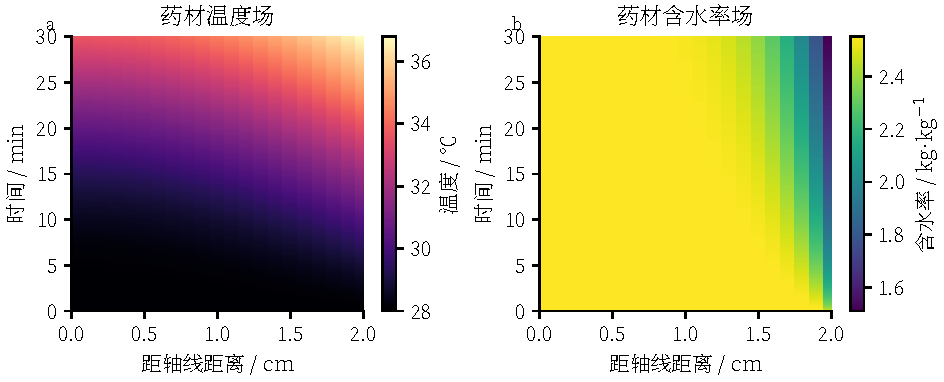
\includegraphics[width=0.92\textwidth]{figures/result_q1_fields.pdf}
\caption{问题一温度场与干基含水率场}
\label{fig:q1-fields}
\end{figure}

将时间步缩小至 \SI{0.125}{s} 后，指定时空点的温度与含水率最大绝对差分别为 \(2.389\times10^{-4}\) \si{\degreeCelsius} 和 \(5.139\times10^{-5}\) \si{kg/kg}。将空间步缩小至 \SI{0.0000625}{m} 后，对应差值分别为 \(2.300\times10^{-5}\) \si{\degreeCelsius} 和 \(3.505\times10^{-4}\) \si{kg/kg}。图 \ref{fig:q1-convergence} 给出两类加密误差，含水率对表面附近的空间分辨率更敏感。

\begin{figure}[htbp]
\centering
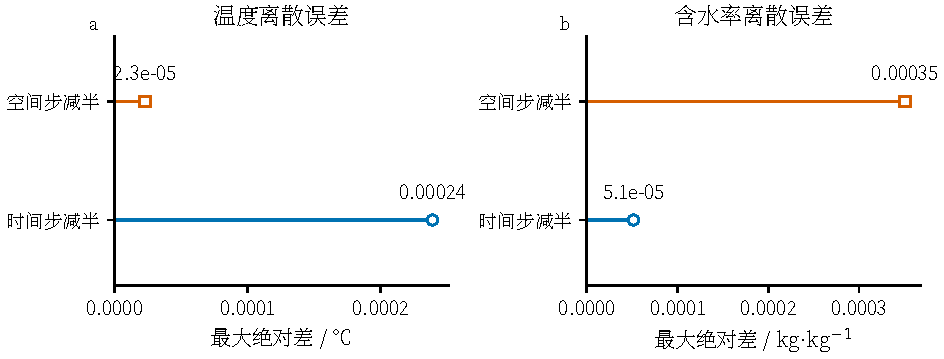
\includegraphics[width=0.92\textwidth]{figures/process_q1_convergence.pdf}
\caption{问题一时间步与空间步加密误差}
\label{fig:q1-convergence}
\end{figure}

由控制体内含水率总变化与表面对流通量分别计算整体平衡，所得相对残差为 \(2.35\times10^{-14}\)。该数值接近双精度浮点运算的舍入尺度，说明离散方程中的内部通量能够在相邻控制体之间抵消，表面通量与域内总量变化保持一致。

\subsection{问题二的模型建立与求解}

\subsubsection{问题二的变物性模型}

问题二继续使用式 \ref{eq:heat-pde} 与式 \ref{eq:moisture-pde}，但物性随局部含水率和温度改变。附录三给出
\begin{align}
\rho(C)&=650+128C,\\
c_p(C)&=1450+2736\frac{C}{C+1},\\
k(C)&=0.21+0.38\frac{C}{C+1},\\
D(C,T)&=2.4\times10^{-3}
\exp\left(-\frac{0.45}{C}\right)
\exp\left(-\frac{3850}{T}\right).
\label{eq:q2-properties}
\end{align}
式 \ref{eq:q2-properties} 中温度 \(T\) 必须使用 K。密度、比热容和导热系数由上一轮含水率更新，扩散系数由当前温度及含水率共同更新。

单个时间层内先求温度方程，再以更新后的温度计算扩散系数并求水分方程。含水率变化会反馈到热物性，故重复上述过程直至温度和含水率同时收敛。控制体几何在问题二和问题三中保持不变，中心条件和表面对流条件沿用式 \ref{eq:heat-center}、式 \ref{eq:heat-surface}、式 \ref{eq:moisture-initial-center} 及式 \ref{eq:moisture-surface}。

\subsubsection{问题二的空气边界}

附件一共有二百四十一条环境记录，时间范围为 \(0\) 至 \SI{14400}{s}，相邻记录间隔均为 \SI{60}{s}。前三小时计算完全落在该范围内，因此各时间步的 \(T_a(t)\) 与 \(C_a(t)\) 都由相邻记录线性插值得到。

长时计算超过附件一范围后，烘房进入恒温干燥阶段。阶段模型把末条记录延拓为常值
\begin{equation}
T_a(t)=\SI{323.315}{K},\qquad
C_a(t)=\SI{0.04986}{kg/kg},
\qquad t>\SI{14400}{s}.
\label{eq:constant-air-boundary}
\end{equation}
式 \ref{eq:constant-air-boundary} 对应 \SI{50.165}{\degreeCelsius}。正式结论需要用末段平均值替换末条记录复算，以检查边界微小波动对终点时长的影响。

\subsubsection{问题二的模型计算结果}

% 待补表 3：0.5、1.0、1.5、2.0、2.5、3.0 h 时，
% r=0、0.5、1、1.5、2 cm 处的温度，数据来自 result2.xlsx。
% 待补表 4：相同时空位置的干基含水率，数据来自 result2.xlsx。
% 待插图：前三小时温度场，标签建议为 fig:q2-temperature。
% 待插图：前三小时含水率场，标签建议为 fig:q2-moisture。
% 待补：变物性耦合迭代的收敛曲线及结果解释。

\subsection{问题三的模型建立与求解}

\subsubsection{问题三的干燥终点模型}

题目要求药材各处含水率低于 \SI{0.15}{kg/kg}。固定半径条件下的结束时刻定义为
\begin{equation}
t_{\mathrm{dry}}^{\mathrm{fixed}}
=
\inf\left\{
t>0:
\max_{0\leq r\leq R}C(r,t)<0.15
\right\}.
\label{eq:fixed-drying-end}
\end{equation}
式 \ref{eq:fixed-drying-end} 直接检查全部径向节点，不预设中心点一定是最大值。

数值求解从问题二的状态连续推进，空气边界按式 \ref{eq:constant-air-boundary} 延拓。每个 \SI{60}{s} 输出时刻计算全域最大含水率，首个满足式 \ref{eq:fixed-drying-end} 的时刻作为离散终点。阈值跨越发生的相邻两个时间层可采用更短时间步复算，以提高终点时间精度。

\subsubsection{问题三的模型计算结果}

% 待补表 5：每隔 6 h 及烘干结束时，
% r=0、0.5、1、1.5、2 cm 处的干基含水率，数据来自 result3.xlsx。
% 待插图：全域最大含水率随时间变化，标签建议为 fig:q3-threshold。
% 待插图：不同半径位置的长时含水率曲线，标签建议为 fig:q3-profiles。
% 待补：固定尺寸烘干时长、阈值附近局部加密结果和单调性核验。

\subsection{问题四的模型建立与求解}

\subsubsection{问题四的移动域模型}

附件二给出 \(R(t)\) 的离散观测值。令
\begin{equation}
x=\frac{r}{R(t)},\qquad 0\leq x\leq 1,
\label{eq:normalized-radius}
\end{equation}
并以 \(\widetilde{T}(x,t)\) 与 \(\widetilde{C}(x,t)\) 表示归一化坐标中的场变量。假定截面作均匀相似收缩，径向材料速度为
\begin{equation}
v_r(r,t)=\frac{rR'(t)}{R(t)}.
\label{eq:material-velocity}
\end{equation}
归一化坐标 \(x\) 随材料点运动，故固定 \(x\) 的时间导数等于物理场的材料导数
\begin{equation}
\left.\frac{\partial \widetilde{u}}{\partial t}\right|_{x}
=
\left.\frac{\partial u}{\partial t}\right|_{r}
+v_r\frac{\partial u}{\partial r},
\label{eq:material-derivative}
\end{equation}
其中 \(u\) 代表温度或干基含水率。

物理域中的温度和含水率守恒式用材料导数表示。将式 \ref{eq:material-derivative} 代入后，网格运动项与材料对流项相消，单位区间上的温度方程为
\begin{equation}
\rho c_p\frac{\partial \widetilde{T}}{\partial t}
=
\frac{1}{xR^2}
\frac{\partial}{\partial x}
\left(
xk\frac{\partial \widetilde{T}}{\partial x}
\right),
\label{eq:moving-heat}
\end{equation}
以及水分方程
\begin{equation}
\frac{\partial \widetilde{C}}{\partial t}
=
\frac{1}{xR^2}
\frac{\partial}{\partial x}
\left(
xD\frac{\partial \widetilde{C}}{\partial x}
\right).
\label{eq:moving-moisture}
\end{equation}
式 \ref{eq:moving-heat} 与式 \ref{eq:moving-moisture} 中的 \(R^{-2}\) 反映扩散距离随收缩而改变。表面热质边界分别写为
\begin{align}
-\frac{k}{R}\left.\frac{\partial\widetilde{T}}{\partial x}\right|_{x=1}
&=h\left[\widetilde{T}(1,t)-T_a(t)\right],\\
-\frac{D}{R}\left.\frac{\partial\widetilde{C}}{\partial x}\right|_{x=1}
&=h_m\left[\widetilde{C}(1,t)-C_a(t)\right].
\label{eq:moving-boundaries}
\end{align}

附录四的物性经验式为
\begin{align}
\rho(C)&=760+90C,\\
c_p(C)&=1850+2150\frac{C}{C+1},\\
k(C)&=0.12+0.20\frac{C}{C+1},\\
D(C,T)&=4.2\times10^{-4}
\exp\left(-\frac{0.30}{C}\right)
\exp\left(-\frac{3850}{T}\right).
\label{eq:q4-properties}
\end{align}
表面边界中的径向导数转换为 \(R^{-1}\partial/\partial x\)。半径在附件二相邻记录间作分段线性插值，晚于 \SI{259200}{s} 时保持 \SI{1.198}{cm}。

归一化截面的平均干基含水率定义为
\begin{equation}
\overline{C}(t)=2\int_0^1\widetilde{C}(x,t)x\,\mathrm{d}x.
\label{eq:mean-moisture}
\end{equation}
对式 \ref{eq:moving-moisture} 积分并代入式 \ref{eq:moving-boundaries}，得到
\begin{equation}
\frac{\mathrm{d}\overline{C}}{\mathrm{d}t}
=-\frac{2h_m}{R(t)}
\left[\widetilde{C}(1,t)-C_a(t)\right].
\label{eq:global-moisture-balance}
\end{equation}
离散计算中可分别由域内含水率变化和表面传质通量计算式 \ref{eq:global-moisture-balance} 两端，其差值用作均匀干固体密度假设下的简化平衡残差。

\subsubsection{问题四的干燥终点模型}

收缩条件下的结束时刻写为
\begin{equation}
t_{\mathrm{dry}}^{\mathrm{shrink}}
=
\inf\left\{
t>0:
\max_{0\leq x\leq 1}\widetilde{C}(x,t)<0.15
\right\}.
\label{eq:shrink-drying-end}
\end{equation}
式 \ref{eq:shrink-drying-end} 与问题三使用相同品质阈值，空间最大值在随材料运动的归一化节点上计算。

题目要求的固定实际距离位置需要由 \(x=r/R(t)\) 映射到当前网格。若某个固定位置已经超出当时半径，则该位置不再作为内部输出点，表格末列改用 \(x=1\) 的表面值。固定尺寸和收缩尺寸结果的比较需同时报告时长差、半径变化及最大含水率控制位置。

\subsubsection{问题四的模型计算结果}

% 待补表 6：每隔 6 h 及烘干结束时，
% r=0、0.5 cm 至当时药材表面处的干基含水率，数据来自 result4.xlsx。
% 待插图：附件二半径曲线及插值结果，标签建议为 fig:q4-radius。
% 待插图：移动域含水率演化，标签建议为 fig:q4-moisture。
% 待插图：固定尺寸与收缩尺寸终点对比，标签建议为 fig:q4-comparison。
% 待补：收缩条件烘干时长、简化平衡残差和坐标映射误差。

\section{模型评价}

\subsection{结构特点}

一维径向控制体直接对应题目要求的空间坐标，环形体积和控制面面积保留了圆柱几何特征。中心控制体的内表面积为零，无需在 \(r=0\) 处直接计算 \(1/r\)，离散后的每个方程仍保持局部守恒。

变物性模型把温度和含水率通过扩散系数及热物性联系起来，能够从预热阶段连续推进到恒温阶段。移动坐标把收缩域转化为固定单位区间，避免反复增删网格，并使问题三和问题四采用同一终点判据。

题面数据直接构成时间边界和半径边界，模型没有为缺失的实验量拟合额外参数。分段线性插值保持原始记录值，结果文件所需的时间和空间分辨率可以由数值网格直接输出。

\subsection{适用边界}

径向模型忽略端面传递，面积比只能说明端部贡献受限，不能证明所有轴向位置都满足相同场分布。靠近端面的温度和含水率可能偏离一维结果，需用二维模型抽样或端部测温数据评估偏差。

问题一把潜热和材料收缩排除在温度方程外，问题二至问题四也用等效扩散系数概括复杂的相变及孔隙输运。若蒸发潜热占热量收支的比例较高，当前温度预测会偏快。药材干基含水率与空气含湿量的基准物质可能不同，直接作差的传质边界需要结合题意和结果范围复核。

长时边界采用附件一末条记录，收缩半径在附件二结束后保持末值。两项延拓都会影响问题三和问题四的干燥终点。正式结果应比较末条记录、末段均值和允许波动区间三种边界，并报告终点时长的变化范围。

% 待补：基于真实结果的误差分析、灵敏度分析和计算复杂度。

\CumcmAIUsed{资料整理、论文结构起草、语言校核和 \LaTeX{} 排版}

\begingroup
\raggedright
\begin{thebibliography}{99}

\bibitem{tzempelikos2015}
TZEMPELIKOS D A, MITRAKOS D, VOUROS A P, et al.
Numerical modeling of heat and mass transfer during convective drying of cylindrical quince slices[J].
Journal of Food Engineering, 2015, 156: 10--21.
DOI: 10.1016/j.jfoodeng.2015.01.017.

\bibitem{silva2014}
DA SILVA W P, E SILVA C M D P S, GAMA F J A.
Estimation of thermo-physical properties of products with cylindrical shape during drying: The coupling between mass and heat[J].
Journal of Food Engineering, 2014, 141: 65--73.
DOI: 10.1016/j.jfoodeng.2014.05.010.

\bibitem{hussain2003}
HUSSAIN M M, DINCER I.
Two-dimensional heat and moisture transfer analysis of a cylindrical moist object subjected to drying: A finite-difference approach[J].
International Journal of Heat and Mass Transfer, 2003, 46(21): 4033--4039.
DOI: 10.1016/S0017-9310(03)00229-1.

\bibitem{liu2020}
刘格含, 王鹏, 吴小华, 等.
农产品热风干燥传热传质数值模拟研究进展[J].
食品工业科技, 2020, 41(22): 342--350, 357.
DOI: 10.13386/j.issn1002-0306.2020010245.

\end{thebibliography}
\endgroup

\clearpage
\begin{appendices}

\section{支撑材料清单}

% 待补：在程序、结果表、正式图和 AI 工具使用详情全部冻结后，
% 按最终提交包中的真实文件名填写支撑材料清单。

\section{计算程序}

% 待补：放入能够从题目附件复现 result1.xlsx 至 result4.xlsx 的完整源程序。
% 程序必须与论文公式、参数、时间步、空间步及最终结果保持一致。

\section{人工核验记录}

% 待补：AI 工具使用详情单独生成 AI工具使用详情.pdf 并放入支撑材料。
% 论文附录只保留组委会要求的文件清单和完整源程序，不写内部质检流程。

\end{appendices}

\end{document}
